% Chapter 1

\chapter{Spectral modelling for astrophysics} % Main chapter title

\label{cha:spectral} % For referencing the chapter elsewhere, use \ref{Chapter1} 

\lhead{Chapter 4. \emph{Spectral modelling}} % This is for the header on each page - perhaps a shortened title

%----------------------------------------------------------------------------------------

\section{Introduction}\label{sec:spe_intro}
For this Chapter, our aim is to connect the determination of sophisticated atomic systems into modelling astrophysical objects, and therefore the collisional-radiative approach is introduced which is dependent on the amount, and the accuracy of atomic data that can be provided. For now we will neglect the contributions from photon-driven processes as a more complex evaluation must be considered. The mean free path is generally much larger than that of electron collisions, and therefore the photon plus material distribution is required at various times where a set of radiative transport equations are to be solved.

In this work we will assume the distribution of free electrons to be that of a Maxwellian,
\begin{equation}\label{eq:spe_max}
f(\nu)= 4\pi \Big(\frac{m}{2\pi k T}\Big)^{3/2}v^{2}e^{-mv^2/2kT}
\end{equation}
where $k$ is Boltzmanns constant, $T$ is the temperature in Kelvin and $v$ is the electron velocity. This is the distribution that has been applied to describe the effective collision strengths in equation (\ref{eq:rmat_ups}).

\section{Collisional radiative modelling}
It is possible to model the excited populations within a particular ion stage, which is known as the isolated-atom approximation. The first step is to consider the populating mechanisms for a chosen system. We recall three types of transitions from Section \ref{sec:many_transition} that can occur. The spontaneous emissions can be characterized by the resulting $A$-values. For the remaining two, we assume energy is transferred from colliding electrons, where specific electron densities are considered later. Assuming the Maxwellian distribution of electron velocities defined in equation (\ref{eq:spe_max}), and using the effective collision strengths in equation (\ref{eq:rmat_ups}) then the excitation rate is defined by,
\begin{equation}\label{eq:spe_erate}
q_{i\rightarrow j }(T) = \frac{2\sqrt{\pi}\alpha c a_0^2}{g_i}\Big(\frac{I_H}{kT}\Big)^{1/2}e^{-\Delta E_{ij}/kT}\Upsilon_{i \rightarrow j}(T).
\end{equation}
$\alpha$, $c$, and $a_0$ are the typical constants for the fine-structure constant, speed of light, and Bohr radius, which results in the units of cm$^3$ s$^{-1}$. $I_H = 13.605698 $ eV is the ionization potential of Hydrogen, $k$ is Boltzmann's constant again in eV/K and $T$ is the temperature in K. Then the de-excitation rate is related by the following equation,
\begin{equation}\label{eq:spe_drate}
q_{j\rightarrow i}(T) = \frac{g_i}{g_j}e^{\Delta E_{ij}/kT}q_{i \rightarrow j}(T).
\end{equation}
There are two limiting cases that we can consider before trying to solve the full problem. The first is when the system is in local thermodynamic equilibrium (LTE), which holds for large electron densities. We introduce $N_k$ as the population in state $\Ket{k}$, which can also be referred to as the number of atoms found in this state. For the LTE approximation, the ratio of populations in two states has a Boltzmann distribution,
\begin{equation}\label{eq:spe_lte}
\frac{N_i}{N_j} = \frac{g_i}{g_j}e^{-\Delta E_{ij}/kT}.
\end{equation}
This tends to happen when collisional processes occur on a timescale much quicker than radiative decay can occur.

The second approximation is the coronal approximation and can be considered as the reverse limitation to LTE, and therefore it holds in the low electron density regime. A population mechanism is still required, and the assumption is that the upper levels can only be populated from the ground state. Due to the low electron densities, the timescale for radiative decay is favourable. Assuming the excited populations are in equilibrium with those in the ground state, it is possible to write, 
\begin{equation}\label{eq:spe_coronal}
N_i = \frac{q_{1\rightarrow i}(T)}{\sum_{j < i}A_{i\rightarrow j}}N_eN_1.
\end{equation}
This is generally not the full scenario, as cascades from higher levels has been neglected, but it is still a useful approximation to consider.

These processes can now be considered in the collisional-radiative regime, where we track how the populations change with respect to electron density and temperature. For now we will just consider one species, and neglect ionization and recombination from the neighbouring stages. The collision matrix then contains all the `driving' mechanisms discussed,
\begin{equation}\label{eq:spe_cmatrix}
C_{ij} = \left\{
  \begin{array}{lr}
   -\sum_{j<i}A_{i\rightarrow j} - N_e\sum_{j\ne i} q_{i\rightarrow j} ~~~~~ (i=j)\\
   A_{j \rightarrow i} + N_eq_{j\rightarrow i} ~~~~~~~~~~~~~~~~~~~~~~~(i<j)\\
   N_eq_{j\rightarrow i} ~~~~~~~~~~~~~~~~~~~~~~~~~~~~~~~~~(i>j)
 \end{array}
 \right.
\end{equation}
which is now a function of both temperature and the electron density, $N_e$, where the temperature dependance is contained through the excitation rate. The diagonal elements track population into a particular state $\Ket{i}$, and the off-diagonal elements track depopulation out of the state. We are left to solve the system of linear equations,
\begin{equation}\label{eq:spe_axb}
\frac{d \boldsymbol{N}}{dt} = \boldsymbol{CN}
\end{equation}
where $\boldsymbol{N}$ is the vector representing the populations of each state. To solve this problem, we assume that the excited state populations are in quasi-static equilibrium with $N_1$, i.e. $d N_i / dt = 0$ for $i > 1$. The solutions we obtain are then represented as a function of $N_1$.

There are a number of useful quantities that can be computed from the above, such as photon emissivity and power-loss coefficients. For now we will focus on the line ratio, which is known to provide useful temperature and density diagnostics of particular astrophysical objects \citep{1988A&A...193..327N}. Since we are taking the ratio of two quantities, the cancellation produces resulting line ratios given as
\begin{equation}\label{eq:spe_lratio}
\mathcal{R} = \frac{I_{j\rightarrow i}}{I_{m \rightarrow n}} = \frac{N_j A_{j\rightarrow i}}{N_m A_{m\rightarrow n}}\frac{\lambda_{nm}}{\lambda_{ij}}
\end{equation}
where each index refer to the occupancy of the state, the $N$'s are the relative populations, the $A$'s are transition probabilities, and the $\lambda$'s are the wavelengths. If we know the ionization rate from a particular level $a$, $S_a$, then we can relate the populations to the ratio of ionizations per photon by,
\begin{equation}\label{eq:spe_sxb}
\mathcal{SXB}_{a,j\rightarrow i} = \frac{N_eS_a}{A_{j\rightarrow i}N_{j}}.
\end{equation}
Where $N_{j}$ is determined by solving the set of equations (\ref{eq:spe_axb}) for the population of level $j$.

%
%%
%%%
%%%%
\begin{figure}
\centering
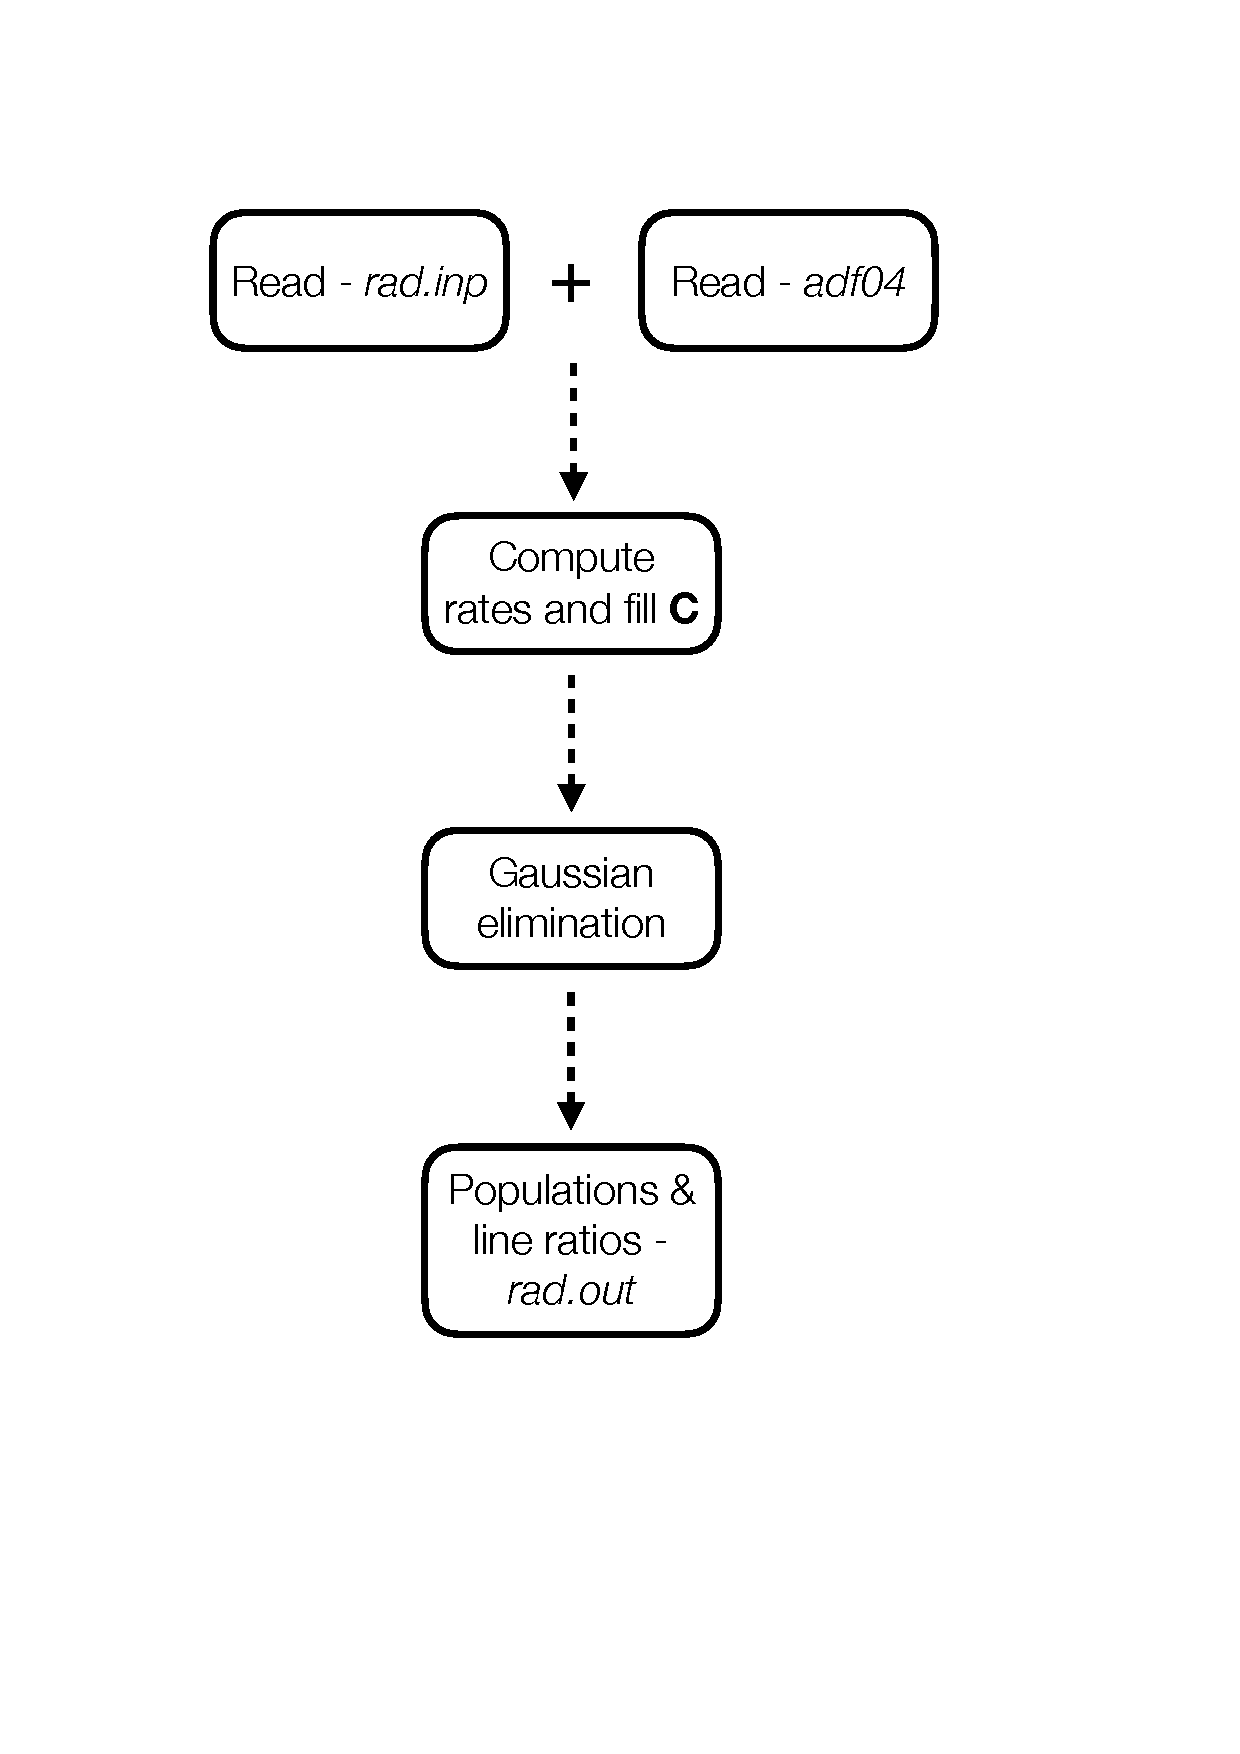
\includegraphics[scale=0.6]{Figures/Spectral/rad_flow.pdf}
\caption{The typical flow of {\sc collr-v1.0} using \textit{rad.inp} and \textit{adf04}. \label{fig:spe_flow}}
\end{figure}
%%%%
%%%
%%
%

\section{Implementation}\label{sec:spe_imp}
We have been able to apply this theory detailed in Section \ref{sec:spe_intro} to develop a simple, working environment. We will refer to the computer code that has been written in {\sc fortran90} as {\sc collr-v1.0}, and a working version is available in Appendix \ref{app:radt}. An advantage to this code is that we have complete control and access over what is included, computed, what can be adjusted, and printed to screen for immediate analysis. This Section details some of the important features to the code and the input required to generate results. We will consider a particular example of Ar$^+$ that has been investigated by \citet{2007JPhB...40.4537G}, and where the corresponding \textit{adf04} input file is available from OPEN-ADAS. An \textit{adf04} input file is a standardized file format that is described in detail on the OPEN-ADAS website. The file typically contains level information with energy values in cm$-1$, effective collision strengths for a number of temperatures, and corresponding $A$-values for each transition. The general flow of {\sc collr-v1.0} is presented in Figure \ref{fig:spe_flow} and a typical run is completed within minutes.

\subsection{Test case: Ar$^+$}
It is clear from the definitions of excitation and de-excitation rates in equation (\ref{eq:spe_erate}) and equation (\ref{eq:spe_drate}) respectively that the order of levels is important. This is not the case however for the symmetric quantities $A_{i\rightarrow j}$ and $\Upsilon_{i\rightarrow j}$. Therefore when reading the effective collision strengths and $A$-values, they must be read as an upper level to a lower level, i.e $j\rightarrow i$.

We also provide the sample input deck (\textit{rad.inp}) below that we have used together with the \textit{adf04} file to generate the results in this Section. For a complete description of all the variables check Appendix A.
\begin{verbatim}
   &COLLINP corrap=1 Nodens=30 notemp=8 grad=0
            sDens=8 fDens=18 IC=0 popt=1 worder=0 
            petol=-2 pops=1 wrngdn=1 wrngup=100000000 /
                       
   &LIRA    line=0 uplev=2 uplevl=1 lolev=3 lolevl=2 
            lopec=1 uppec=3 ppec=0 /
\end{verbatim}
In {\sc collr-v1.0} there are two important and essential namelists that must be included. \texttt{\&COLLINP} is mainly concerned with input and reading, and the second, \texttt{\&LIRA} which stands for \texttt{LI}ne \texttt{RA}tio is concerned with output and printing. The majority of these variables are defaulted at the beginning of the code to produce minimal output if they are not specified in these namelists.

The number of temperatures must be provided by the variable \texttt{notemp}. If only a subset of temperatures are required, \texttt{mintmp} and \texttt{maxtmp} can be included such that $1\le \texttt{mintmp} \le \texttt{maxtmp} \le \texttt{notemp}$. As this operation is relatively quick we recommend ignoring these variables. A user input, logarithmic grid of electron densities are then initialized through \texttt{Nodens>2} where $10^{\texttt{sDens}} \le N_e \le 10^{\texttt{fDens}}$.

%
%%
%%%
%%%%
\begin{figure}
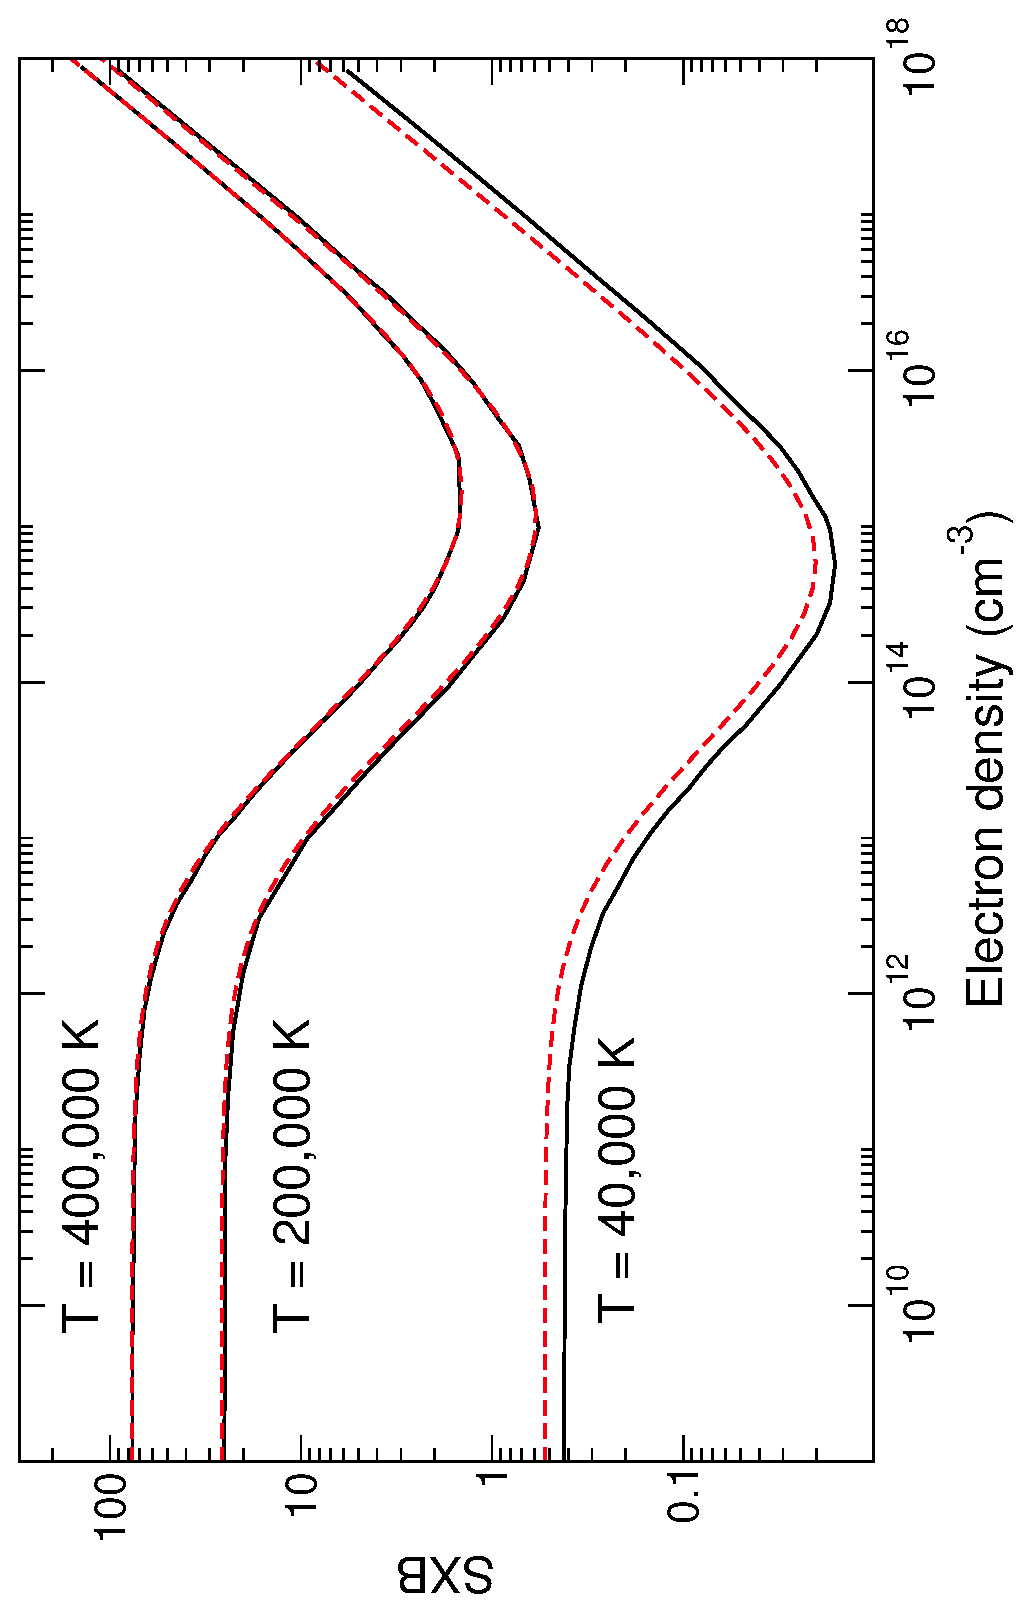
\includegraphics[scale=0.55,angle=-90]{Figures/Spectral/comparison1.eps}
\caption{The $\mathcal{SXB}_{1,3\rightarrow 2}$ ratio for Case 1 as a function of the electron density for three temperatures $T=40,000$ K, $T=200,000$ K, and $T=400,000$ K. The solid black curves are the results from \citet{2007JPhB...40.4537G}, and the dashed red curves are generated with the same input from the {\sc collr-v1.0} computer code. \label{fig:spe_sxb1}}
\end{figure}
%%%%
%%%
%%
%

%
%%
%%%
%%%%
\begin{figure}
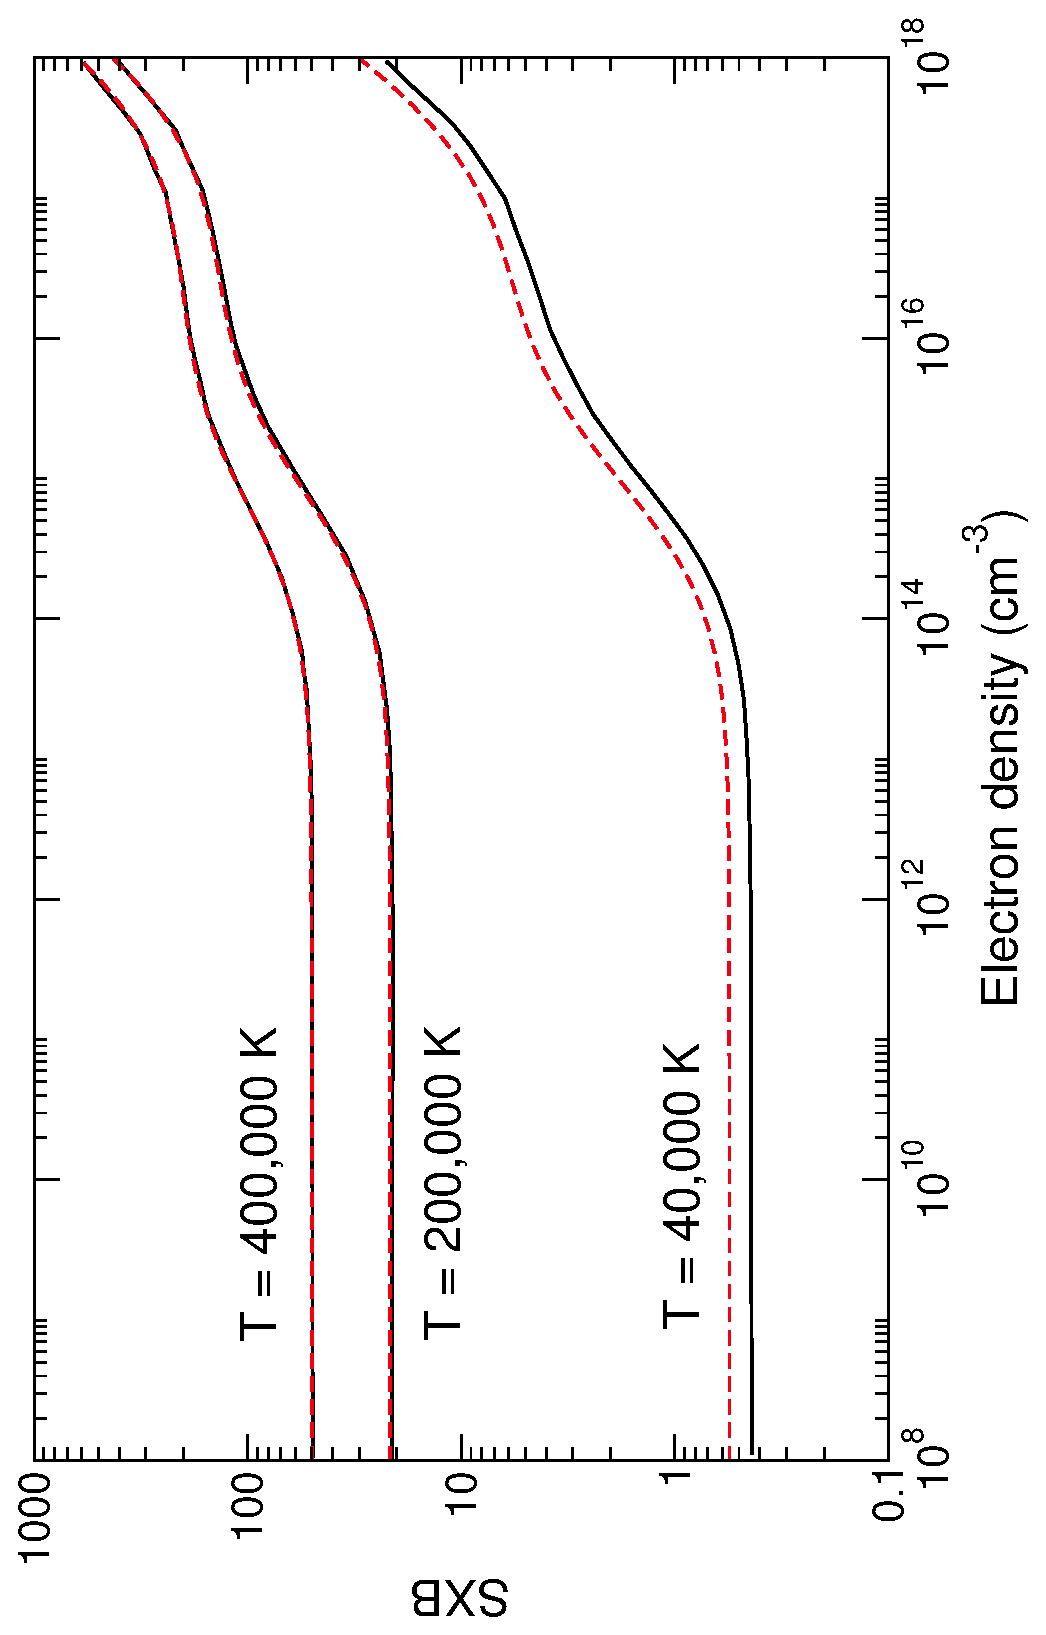
\includegraphics[scale=0.55,angle=-90]{Figures/Spectral/comparison2.eps}
\caption{The $\mathcal{SXB}_{1,3\rightarrow 2}$ ratio for Case 2 as a function of the electron density for three temperatures $T=40,000$ K, $T=200,000$ K, and $T=400,000$ K. The solid black curves are the results from \citet{2007JPhB...40.4537G}, and the dashed red curves are generated with the same input from the {\sc collr-v1.0} computer code. \label{fig:spe_sxb2}}
\end{figure}
%%%%
%%%
%%
%

A useful test is to consider the two limiting cases; LTE (high density), and the coronal approximation (low density), for particular line ratios in equation (\ref{eq:spe_lratio}). Therefore, by applying the two equations (\ref{eq:spe_lte}) and (\ref{eq:spe_coronal}), the values are computed for all temperatures by setting the flags \texttt{corrap=1} and \texttt{lte=1}.

Finally, we can look at particular photon emissivity coefficients over a range of electron temperatures and densities. This is initialized by setting $\texttt{ppec} = 1$, to calculate between an upper ($\texttt{uppec}$), and lower ($\texttt{lopec}$) state. It is also possible to calculate certain line ratios from equation (\ref{eq:spe_lratio}) by setting the following variables,
\[
\mathcal{R} = \frac{I_{\texttt{uplev}\rightarrow \texttt{uplevl}}}{I_{\texttt{lolev} \rightarrow \texttt{lolevl}}} = \frac{N_{\texttt{uplev}} A_{\texttt{uplev}\rightarrow \texttt{uplevl}}}{N_{\texttt{lolev}} A_{\texttt{lolev}\rightarrow \texttt{lolevl}}}\frac{\lambda_{\texttt{lolevl,lolev}}}{\lambda_{\texttt{uplevl,uplev}}} ~~~~~~~ {\rm if} ~~~ \texttt{line = 1}.
\]
To improve and validate the current set of codes, we look at two, three levels systems from the work carried out by \citet{2007JPhB...40.4537G}:\\\\
Case 1: ~~~level 1 - 3p$^5$ $^2$P ~~~level 2 - 3p$^4$4p $^4$D$^{\rm o}$  ~~~level 3 - 3p$^4$4s $^4$P\\
Case 2: ~~~level 1 - 3p$^5$ $^2$P ~~~level 2 - 3p$^4$4p $^2$D$^{\rm o}$ ~~~level 3 - 3p$^4$4s $^2$P.\\\\
We therefore use the input test case of \textit{rad.inp} for Case 1 and Case 2, and compute the $\mathcal{SXB}_{1,3\rightarrow 2}$ ratio from equation (\ref{eq:spe_sxb}). The results for the corresponding cases are shown in Figures \ref{fig:spe_sxb1} and \ref{fig:spe_sxb2} as a function of the electron density for three temperatures of $T=40,000$ K, $T=200,000$ K, and $T=400,000$ K. There is excellent agreement between the magnitude of results and dominant features between the two calculations, with only slight deviation for the low temperature ratio of $T=40,000$ K.
\newpage

\section{Radiative and dielectronic recombination rate coefficients}\label{sec:spe_rranddr}
These astrophysical plasma, as well as laboratory plasma often require descriptions such as those in Section \ref{sec:spe_imp} for ionization and recombination processes. Numerous investigations have been carried out for these recombination processes in low density regimes \citep{1982ApJS...48...95S, 1985A&AS...60..425A, 1991A&A...251..680P}, but more recently work has been focused towards expanding to study NLTE regimes \citep{2003A&A...406.1151B, 2006ApJ...651L..73B, 2005ApJS..158...80N}.

Another extremely important mechanism to consider is determining the ionization balance with neighbouring ion stages, i.e. extending the isolated atom approximation. Currently, {\sc collr-v1.0} does not have the capability to include ionization and recombination rates during the collisional-radiative process.

The definition for the radiative recombination process is the capture of an electron into some bound state. This is precisely the reverse process defined in equation (\ref{eq:rmat_basicphoto}), so we can write
\begin{equation}\label{eq:rmat_basicre}
\begin{split}
& ~~~~~~~~~~~~~~ \tiny{\circled{1}}\\
& h\nu+ X_i^{q+} \leftarrow X_f^{(q+1)+} +e^-\\
& ~~~\tiny{\circled{2}}\nwarrow ~~~~~~~~~~~~~~~~~\swarrow \tiny{\circled{2}} \\
& ~~~~~~~~~~~~(X_y^{q+})^*
\end{split}
\end{equation}
We refer to the process in 1) as radiative recombination (RR) and 2) as dielectronic recombination (DR). Therefore, the $R$-matrix technique provides an approach for calculating the partial recombination rates for a specific transition through all its autoionization states. We write this partial contribution from an initial electron plus ion system to some final bound state as,
\begin{equation}\label{eq:spe_partialrate}
\tilde{\alpha}^{P}_{f\rightarrow i} = \alpha^{RR}_{f\rightarrow i} + \sum_y\alpha^{DR}_{y\rightarrow i}.
\end{equation}
We do not explicitly calculate the total rate, but it can be obtained by summing over all final bound states defined by equation (\ref{eq:spe_partialrate}),
\[
\alpha^{Tot}_f = \sum_i\tilde{\alpha}^{P}_{f\rightarrow i}.
\]
By assuming detailed balance and LTE from equation (\ref{eq:spe_lte}), it is possible to write the photoionization cross-sections in terms of the recombination cross-sections by appling the Milne relation,
\begin{equation}\label{eq:spe_milne}
\frac{\sigma^{r}_{f\rightarrow i}}{\sigma^p_{i\rightarrow f}}= \frac{g_i}{g_f}\frac{(\alpha E)^2}{4\epsilon}.
\end{equation}
$\alpha$ with no subscripts is the fine-structure constant, $E$ is the photon energy in Rydbergs, and $\epsilon$ is the kinetic energy of the electron in Rydbergs. By describing the distribution of electron velocities as Maxwellian in equation (\ref{eq:spe_max}), it is possible now to compute the formal definition for the rates defined in equation (\ref{eq:spe_partialrate}),
\begin{equation}\label{eq:spe_formalrate}
\tilde{\alpha}^P_{f\rightarrow i} = \int\frac{g_i}{2g_f}(\alpha E)^2f(v)\sigma^p_{i\rightarrow f}d\epsilon.
\end{equation}
%
%%
%%%
%%%%
\begin{figure}
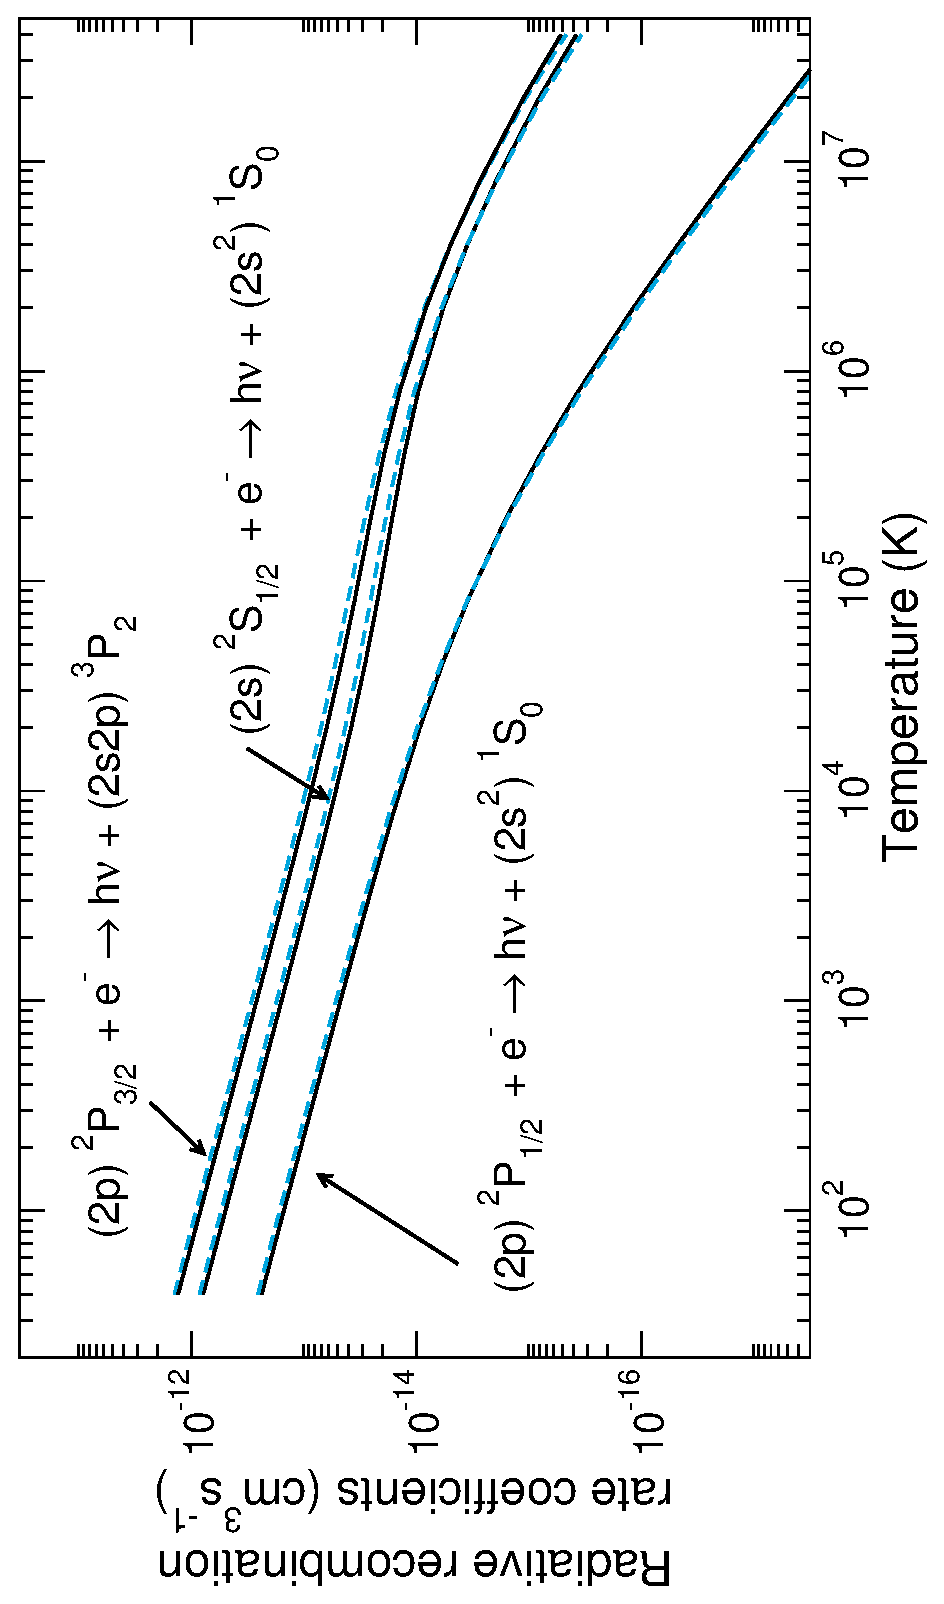
\includegraphics[scale=0.54,angle=-90]{Figures/Spectral/rates/be-like/total.eps}
\caption{Radiative recombination rates in cm$^3$s$^{-1}$ as a function of electron temperature in K. The three transitions plotted are $\tilde{\alpha}^P_{1\rightarrow 1} \equiv$ 2s $^2$S$_{1/2}$ + e$^-$ $\rightarrow$ $h\nu$ + 2s$^2$ $^1$S$_0$, $\tilde{\alpha}^P_{2\rightarrow 1} \equiv$ 2p $^2$P$_{1/2}^{\rm o}$ + e$^-$ $\rightarrow$ $h\nu$ + 2s$^2$ $^1$S$_0$, and $\tilde{\alpha}^P_{3\rightarrow 4} \equiv$ 2p $^2$P$_{3/2}^{\rm o}$ + e$^-$ $\rightarrow$ $h\nu$ + 2s2p $^3$P$_2^{\rm o}$. The black curve are the results from \citet{2006ApJS..167..334B} and the blue dashed curves are the present results.\label{fig:spe_boron}}
\end{figure}
%%%%
%%%
%%
%
where $f(v)$ is the Maxwellian distribution and the integration is over all kinetic energies of the scattered electron. We consider standard integration techniques with data produced using the computer code {\sc autostructure}. The photoionization cross-sections obtained from OPEN-ADAS are transformed to recombination cross-sections by equation (\ref{eq:spe_milne}), which are then used to determine the recombination rates from equation (\ref{eq:spe_formalrate}). We present in Figure \ref{fig:spe_boron} three transitions of Be-like Boron for,\\
$\tilde{\alpha}^P_{1\rightarrow 1} \equiv$ 2s $^2$S$_{1/2}$ + e$^-$ $\rightarrow$ $h\nu$ + 2s$^2$ $^1$S$_0$, \\
$\tilde{\alpha}^P_{2\rightarrow 1} \equiv$ 2p $^2$P$_{1/2}^{\rm o}$ + e$^-$ $\rightarrow$ $h\nu$ + 2s$^2$ $^1$S$_0$,\\
$\tilde{\alpha}^P_{3\rightarrow 4} \equiv$ 2p $^2$P$_{3/2}^{\rm o}$ + e$^-$ $\rightarrow$ $h\nu$ + 2s2p $^3$P$_2^{\rm o}$,\\\\
and compare the blue dashed curves from equation (\ref{eq:spe_formalrate}) with the published rates of \citet{2006ApJS..167..334B} with excellent agreement.

It is therefore possible to compute the partial recombination rates defined by equation (\ref{eq:spe_formalrate}) directly from the photoionization cross-sections that we calculate in equation (\ref{eq:rmat_totphoto}).





%----------------------------------------------------------------------------------------


